\chapter*{basic functions or methods for numerical matrices}\addcontentsline{toc}{chapter}{basic functions or methods for numerical matrices}
\hypertarget{basicnumarrays}{}
\begin{quote}
\noindent
\hyperlink{zeros}{zeros},\hyperlink{ones}{ones} - build matrices of zeros or ones \\
\hyperlink{eye}{eye} - identity matrix or matrix of canonical application between 2 vector spaces \\
\hyperlink{tril}{tril}, \hyperlink{triu}{triu} - extract lower or upper triangle part of a matrix \\
\hyperlink{diag}{diag} - extract a diagonal of a matrix or build a diagonal matrix from a vector \\
\hyperlink{set_diag}{set\_diag} - (method) set a diagonal of a matrix \\
\hyperlink{sum}{sum},\hyperlink{prod}{prod} - sum and product of matrix elements \\
\hyperlink{cumsum}{cumsum},\hyperlink{cumprod}{cumprod} - cumulative sum and product of matrix elements \\
\hyperlink{diff}{diff} - difference of a vector or a matrix \\
\hyperlink{min}{min} - minimum of matrix elements or minimum of 2 or more matrices \\
\hyperlink{max}{max} - maximum of matrix elements or maximum of 2 or more matrices \\
\hyperlink{minmax}{minmax} - both minimum and maximum of matrix elements\\
\hyperlink{dot}{dot} - scalar product of 2 vectors (or matrices) \\
\hyperlink{cross}{cross} - cross product of 2 vectors \\
\hyperlink{scale_rows}{scale\_rows} - multiply each row of a matrix by a different scalar \\
\hyperlink{scale_cols}{scale\_cols} - multiply each column of a matrix by a different scalar \\
\hyperlink{blas_axpy}{blas\_axpy} -  add to a vector (or a matrix) another vector (or matrix) times a scalar\\ 
\hyperlink{blas_ger}{blas\_ger} -  matrix rank one update\\ 
\hyperlink{ndgrid}{ndgrid} - arrays for multidimensional function evaluation on grid \\
\hyperlink{linspace}{linspace} - uniform mesh/partition of a segment \\
\hyperlink{logspace}{logspace} - logarithmically spaced vector \\
\end{quote}
 
\mansection{zeros, ones}
\begin{mandesc}
  \short{zeros}{matrix of zeros}\\ 
  \short{ones}{matrix of ones}
\end{mandesc}
%-- Calling sequence section
\begin{calling_sequence}
\begin{verbatim}
A = zeros(n ,like=obj,type=string)
A = zeros(m,n,like=obj,type=string)
A = zeros(dims,like=obj,type=string)
A = ones(n,like=obj,type=string)
A = ones(m,n,like=obj,type=string)
A = ones(dims,like=obj,type=string)
\end{verbatim}
\end{calling_sequence}
%-- Parameters
\begin{parameters}
  \begin{varlist}
    \vname{m,n}: integers
    \vname{dims}: vector of integers of length 1 or 2.
    \vname{A}: matrix of zeros or ones.
    \vname{like}: optional parameter which value gives the type of the result.
    \vname{type}: a string giving the type of the result. It can be \verb+"double"+ or \verb+"m"+ for 
    scalar matrices, \verb+"boolean"+ or \verb+"b"+ for boolean matrices or it can be a string giving 
    an integer type. (See \manlink{IMat}{IMat}).
  \end{varlist}
\end{parameters}

\begin{mandescription}
\verb+zeros(n)+ is the same as \verb+zeros(n,n)+. If \verb+dims+ is a vector of length 2, 
with $dims_1 = m$ and $dims_2 = n$ then \verb+zeros(m,n)+ and  \verb+zeros(dims)+ are equivalent 
and output a $m \times n$ matrix of zeros. The second form could be useful to get a matrix of 
zeros of same size as another matrix $M$ using:
\begin{verbatim}
    A = zeros(size(M))
\end{verbatim}

The \verb+ones+ function works similarly but outputs a matrix of ones.

An optional parameters can be given to specify the type of the result which can 
be a scalar, or a boolean, or an integer matrix. For example, to get a matrix of 
zeros of same size and type as matrix $M$ on can use:
\begin{verbatim}
    A = zeros(size(M),like=M);
\end{verbatim}

\end{mandescription}

%--example 
\begin{examples}
\begin{mintednsp}{nsp}
A = ones(2,3) 
B = zeros(1,4)
C = zeros(3,0)
D = ones(0,2)
C*D
A = ones(2,3,like=%t);
A = ones(2,3,type='int64');
\end{mintednsp} 

\end{examples}

%-- see also
\begin{manseealso}
\manlink{eye}{eye}, \manlink{repmat}{repmat}
\end{manseealso}


\mansection{eye}
\begin{mandesc}
  \short{eye}{identity matrix or matrix of canonical application between 2 vector spaces} 
\end{mandesc}
%-- Calling sequence section
\begin{calling_sequence}
\begin{verbatim}
I = eye(n)
I = eye(m,n)
I = eye(dims)
\end{verbatim}
\end{calling_sequence}
%-- Parameters
\begin{parameters}
  \begin{varlist}
    \vname{m,n}: integers
    \vname{dims}: vector of integers of length 1 or 2.
    \vname{A}: resulting matrix.
  \end{varlist}
\end{parameters}

\begin{mandescription}
\verb+eye(n)+ is the same than \verb+eye(n,n)+ and output the identity matrix of the $n$ dimensional
vector space. More generally \verb+eye(m,n)+ output the matrix of the canonical application $J$ from
the $n$ dimensional vector space to the  $m$ dimensional vector space: 
$$
x = \left[ x_1 ; x_2 ; \dots ; x_n \right]  \longmapsto  J x = 
\left\{ 
\begin{array}{l} 
     \left[ x_1 ; x_2 ; \dots ; x_m \right] \mbox{ if } m \le n \\ \left[ x_1 ; x_2 ; \dots ; x_n ; 0 ; \dots ; 0 \right] \mbox{ otherwise }
\end{array} 
\right.
$$
With $m=3$ and $n=4$ we get:
$$
    I = \left( \begin{array}{cccc} 1 & 0 & 0 & 0 \\ 0 & 1 & 0 & 0 \\ 0 & 0 & 1 & 0
      \end{array} \right)
$$
\verb+eye(dims)+ with $dims_1 = m$ and $dims_2 = n$ is the same than  \verb+eye(m,n)+. If you want
such a matrix of same size than another matrix $M$ use: 
\begin{verbatim}
   I = eye(size(M))
\end{verbatim}

\end{mandescription}


%--example 
\begin{examples}
\begin{program}\HCode{I = eye(2,3) \Hnewline
I = eye(0,3)}
\end{program} 

\end{examples}

%-- see also
\begin{manseealso}
\manlink{zeros}{zeros}, \manlink{ones}{ones}
\end{manseealso}


\mansection{tril and triu}
\begin{mandesc}
  \short{tril}{extract a lower triangle of the matrix}\\
  \short{triu}{extract an upper triangle of the matrix}
\end{mandesc}
%-- Calling sequence section
\begin{calling_sequence}
\begin{verbatim}
  B = tril(A)
  B = tril(A,k)
  
  B = triu(A)
  B = triu(A,k)
\end{verbatim}
\end{calling_sequence}
%-- Parameters
\begin{parameters}
  \begin{varlist}
    \vname{A}: matrix (full or sparse).
    \vname{k}: optional argument, must be an integer (default is $0$)
    \vname{B}: matrix (full or sparse).
  \end{varlist}
\end{parameters}
\begin{mandescription}
  \verb+tril(A,k)+ extracts the lower triangle of the matrix $A$ ``until'' the diagonal number $k$
  (this one comprised) while the \verb+triu(A,k)+ extracts the upper triangle ``from'' the  diagonal
  number $k$. The matrix element $A_{i,j}$ is located on the diagonal number $j-i$. So main 
  diagonal is numbered $0$, the diagonal number $1$ and $-1$ are respectively located just 
  upper and under the main diagonal, etc...
  $$
  \includegraphics[width=8cm]{diagonal} 
  $$
  More precisely, if $A$ is a $m \times n$ then   $B = tril(A,k)$ and $C=triu(A,k)$ are both $m \times n$ matrices and:

%%   $$
%%   \begin{array}{l}
%%     B_{i,j} = \left\{ \begin{array}{l} A_{i,j} \mbox{ if } j-i \le k \\
%%       0    \mbox{ otherwise}
%%     \end{array} \right.   \\
%%     C_{i,j} = \left\{ \begin{array}{l} A_{i,j} \mbox{ if } j-i \ge k \\
%%       0    \mbox{ otherwise}
%%     \end{array} \right. 
%%   \end{array}
%%   $$

  \begin{align*}
  B_{i,j} &= 
  \begin{cases}
    A_{i,j} & \text{ if $j-i \le k$}, \\
    0  &  \text{ otherwise.}
  \end{cases} \\
  C_{i,j} &= 
  \begin{cases}  A_{i,j} &\text{ if $j-i \ge k$}, \\
      0   & \text{ otherwise}.
  \end{cases}
  \end{align*}

\end{mandescription}
%--example 
\begin{examples}
  \begin{program}\HCode{A=rand(4,5) \Hnewline
      tril(A) \Hnewline
      tril(A,-1) \Hnewline
      tril(A,1) \Hnewline
      triu(A) \Hnewline
      triu(A,-1) \Hnewline
      triu(A,1)}
  \end{program}
\end{examples}

%-- see also
\begin{manseealso}
  \manlink{diag}{diag}
\end{manseealso}


\mansection{diag}
\begin{mandesc}
  \short{diag}{extract a diagonal of a matrix or build a diagonal matrix from a vector}
\end{mandesc}
%-- Calling sequence section
\begin{calling_sequence}
\begin{verbatim}
  // form 1
  A = diag(v)
  A = diag(v,k)

  // form 2
  v = diag(A)
  v = diag(A,k)
\end{verbatim}
\end{calling_sequence}
%-- Parameters
\begin{parameters}
  \begin{varlist}
    \vname{A}: matrix (full or sparse)
    \vname{v}: vector (full or sparse)
    \vname{k}: optional argument, must be an integer (default is $0$)
  \end{varlist}
\end{parameters}

\begin{mandescription}

  This function has two different behaviors depending if the first argument is a vector
  (call it form 1) or a matrix which is not a vector (called form 2).
  For both forms of this function, the optional argument $k$ have the same meaning and
 corresponds to the choosen diagonal number (see definition and a figure on the 
 \manlink{tril, triu}{tril} help page).

\begin{itemize}
\item \itemdesc{form 1}
   We get this behavior when the first argument, says \verb+v+ is detected as a vector, that is,
 it is a $m \times n$ matrix (full or sparse) with $m$ or $n$ equal to $1$. In this case the
 output  \verb+A+ is a matrix (full or sparse) with the $k$ th diagonal filled with the vector
 \verb+v+. If  \verb+v+ has $mn$ elements, we get a $p \times p$ (square) matrix (full or sparse)
 with $p=mn + | k |$. Note that it can be more efficient to use the \manlink{set_diag}{set_diag}
 method.
   
\item \itemdesc{form 2}
  To have this behavior, the first argument, says \verb+A+ should have been detected as 
a  $m \times n$ matrix (full or sparse) with both $m$ and $n$ differents of $1$. In this 
case the function extract the $k$ th diagonal of the matrix $A$ as a column vector (full or sparse).
\end{itemize}

\itemdesc{Remark:} When $v$ is a sparse vector, we get a sparse matrix $A$ and conversely.


\end{mandescription}

%--example 
\begin{examples}
\paragraph{first form examples}
  \begin{program}\HCode{v=rand(4,1) \Hnewline
diag(v) \Hnewline
diag(v,-1) \Hnewline
diag(v,1)\Hnewline
// build the 1d discrete laplacien matrix (as a full matrix)\Hnewline
n = 5;\Hnewline
v = ones(n-1,1);\Hnewline
A = 2*eye(n) - diag(v,1) + diag(v,-1)\Hnewline
// build the 1d discrete laplacien matrix (as a sparse matrix)\Hnewline
n = 5;\Hnewline
v = sparse(ones(n-1,1));\Hnewline
A = 2*speye(n,n) - diag(v,1) + diag(v,-1)}
\end{program}

\paragraph{second form examples}
  \begin{program}\HCode{A=rand(4,5) \Hnewline
      diag(A) \Hnewline
      diag(A,-1) \Hnewline
      diag(A,1)}
  \end{program}
\end{examples}

%-- see also
\begin{manseealso}
 \manlink{set_diag}{set_diag}, \manlink{eye}{eye}, \manlink{tril}{tril}, \manlink{triu}{triu}
\end{manseealso}


\mansection{set\_diag}
\begin{mandesc}
  \short{set_diag}{set a diagonal of a matrix}
\end{mandesc}
%-- Calling sequence section
\begin{calling_sequence}
\begin{verbatim}
  A.set_diag[v]
  A.set_diag[v,k]
\end{verbatim}
\end{calling_sequence}
%-- Parameters
\begin{parameters}
  \begin{varlist}
    \vname{A}: any kind of matrix
    \vname{v}: vector or scalar (of same type than A)
    \vname{k}: optional argument, the diagonal number (default is $0$)
  \end{varlist}
\end{parameters}

\begin{mandescription}

  This function sets the given diagonal $k$ (0 by default) of a matrix 
with either a vector (which must have as many elements as the given 
diagonal) or with a scalar (the given diagonal is filled with the
scalar).

Remarks:  
\begin{itemize}
\item The matrix element $A_{i,j}$ is located on the diagonal number $j-i$. So main 
diagonal is numbered $0$, the diagonal number $1$ and $-1$ are respectively located just 
upper and under the main diagonal, etc...
  $$
  \includegraphics[width=8cm]{\mansrc basicnumarrays/diagonal} 
  $$

\item For a sparse matrix, argument $v$ can be given also using a full vector (or scalar).

\end{itemize}

\end{mandescription}

%--example 
\begin{examples}
\begin{Verbatim}
A = zeros(5,5)
A.set_diag[2]; A.set_diag[-1,1];  A.set_diag[-1,-1]; 
print(A)

// same example with a sparse matrix
A = sp_create(5,5)
A.set_diag[2]; A.set_diag[-1,1];  A.set_diag[-1,-1]; 
print(A)

// an example with a IMat
A = imat_create(4,6)
for k=-3:5; A.set_diag[m2i(k),k]; end
print(A)

// an example with a string matrix
A = smat_create(3,3)
A.set_diag["a",-2]
A.set_diag[["b","c"],-1]; 
A.set_diag[["d","e","f"],0]; 
A.set_diag[["g","h"],1]; 
A.set_diag[["i"],2]; 
print(A)
\end{Verbatim}
\end{examples}

%-- see also
\begin{manseealso}
  \manlink{diag}{diag}, \manlink{tril}{tril}, \manlink{triu}{triu}
\end{manseealso}


\mansection{sum and prod}
\begin{mandesc}
  \short{sum}{sum of matrix elements}\\ % @mandesc@
  \short{prod}{product of matrix elements}\\ % @mandesc@
\end{mandesc}
%-- Calling sequence section
\begin{calling_sequence}
\begin{verbatim}
  B=sum(A,mode)  
  B=prod(A,mode)  
  B=sum(A,dim=mode) 
  B=prod(A,dim=mode)  
\end{verbatim}
\end{calling_sequence}
%-- Parameters
\begin{parameters}
  \begin{varlist}
    \vname{A,B}: matrices.
    \vname{mode}: A string chosen among \verb+'M'+, \verb+'m'+, \verb+'full'+, \verb+'FULL'+, \verb+'row'+,
    \verb+'ROW'+, \verb+'col'+, \verb+'COL'+ or an non ambiguous abbreviation or an integer. 
    This argument is optional and if omitted 'full' is assumed.
  \end{varlist}
\end{parameters}
\begin{mandescription}
  \verb+sum+ (resp. \verb+prod+) gives the sum (resp. the product) of the elements of the given matrix
  argument \verb+A+. 
  The second argument gives the dimension to be used for performing the sum (resp product) of elements.
  \begin{itemize}
    \item 'full' or 0  $$B= \sum_{i,j} A_{i,j} \quad \left(\text{resp. } \prod_{i,j} A_{i,j} \right)$$ and thus gives a scalar.
    \item 'row' or 1  $$B_j = \sum_{i} A_{i,j}\quad \left(\text{resp. } \prod_{i} A_{i,j} \right)$$ and thus gives a row vector.
    \item 'col' or 2  $$B_i = \sum_{j} A_{i,j}\quad \left(\text{resp. } \prod_{j} A_{i,j}\right)$$ and thus gives a column vector.
    \item 'm' is the sum (resp. product) along the first non singleton dimension of the given matrix 
      for Matlab compatibility. 
  \end{itemize}
\end{mandescription}
%--example 
\begin{examples}
  \begin{program}\HCode{A=rand(4,5) \Hnewline
      sum(A,'c'); \Hnewline
      // boolean matrix \Hnewline
      sum(A>=0.5,'c');\Hnewline
      prod(1:5,'m') \Hnewline
      // sparse matrix 
      sum(sparse(rand(4,6)),'r')  }
  \end{program}
\end{examples}
%-- see also
\begin{manseealso}
  \manlink{cumsum}{cumsum}  \manlink{cumprod}{cumprod} 
\end{manseealso}


\mansection{cumsum and cumprod}
\begin{mandesc}
  \short{cumsum}{cumulative sum of matrix elements}\\ % @mandesc@
  \short{cumprod}{cumulative product of matrix elements}\\ % @mandesc@
\end{mandesc}
%-- Calling sequence section
\begin{calling_sequence}
\begin{verbatim}
  B=cumsum(A,mode)  
  B=cumprod(A,mode)  
  B=cumsum(A,dim=mode) 
  B=cumprod(A,dim=mode)  
\end{verbatim}
\end{calling_sequence}
%-- Parameters
\begin{parameters}
  \begin{varlist}
    \vname{A,B}: matrices.
    \vname{mode}: A string chosen among \verb+'M'+, \verb+'m'+, \verb+'full'+, \verb+'FULL'+, \verb+'row'+,
    \verb+'ROW'+, \verb+'col'+, \verb+'COL'+ or an non ambiguous abbreviation or an integer. 
    This argument is optional and if omitted 'full' is assumed.
  \end{varlist}
\end{parameters}
\begin{mandescription}
  \verb+cumsum+ (resp. \verb+cumprod+) gives the cumulative sum (resp. product) of the 
  elements of the given matrix argument \verb+A+. 
  The second argument gives the dimension to be used for performing the cumsum (resp product) of entries.       
  \begin{itemize}
  \item 'full' or 0 \verb+B+ and \verb+A+ have the same size and 
    $$B_{i,j} = \sum_{k+(l-1)m \le i+(j-1)m } A_{k,l} \quad \left( \text{resp. } \prod_{k+(l-1)m \le i+(j-1)m } A_{k,l} \right)$$ 
    where $m$ is the number of rows of \verb+A+
  \item 'row' or 1  \verb+B+ and \verb+A+ have the same size and 
    $$B_{i,j} = \sum_{k\le i} A_{k,j}\quad \left(\text{resp. }  \prod_{k\le i} A_{k,j}\right) \,. $$     
  \item 'col' or 2  \verb+B+ and \verb+A+ have the same size and 
    $$B_{i,j} = \sum_{l\le j} A_{i,l} \quad \left(\text{resp. }  \prod_{l\le j} A_{i,l}  \right) \,. $$     
  \item 'm' is the cumulative sum (resp. product) along the first non singleton dimension of the given matrix 
    for Matlab compatibility. 
  \end{itemize}
\end{mandescription}
%--example 
\begin{examples}
  \begin{mintednsp}{nsp}
    A=rand(4,5) 
    cumsum(A,dim='c'); 
    // boolean matrix 
    cumsum(A>=0.5,dim='c');
    cumprod(1:5,dim='m') 
    // sparse matrix 
    // cumsum(sparse(rand(4,6)),dim='r')
  \end{mintednsp}
\end{examples}
% -- see also
\begin{manseealso}
  \manlink{sum}{sum}  \manlink{prod}{prod} 
\end{manseealso}


\mansection{diff}
\begin{mandesc}
  \short{diff}{difference of a vector or a matrix}
\end{mandesc}
%-- Calling sequence section
\begin{calling_sequence}
\begin{verbatim}
  d=diff(x)  
  d=diff(x,dim=dimval, order=orderval)  
  d=diff(x,dimval,orderval)
\end{verbatim}
\end{calling_sequence}
%-- Parameters
\begin{parameters}
  \begin{varlist}
    \vname{x}: numerical vector or matrix
    \vname{dimval}: A string chosen among \verb+'M'+, \verb+'m'+, \verb+'full'+, \verb+'FULL'+, \verb+'row'+,
    \verb+'ROW'+, \verb+'col'+, \verb+'COL'+ or an non ambiguous abbreviation or an integer. 
    This argument is optional and if omitted 'full' is assumed.
    \vname{orderval}: a non negative integer (default is 1)   
  \end{varlist}
\end{parameters}
\begin{mandescription}
  \verb+diff+ computes the difference of a vector \verb+x+ which is defined as follows~:
$$ d_1 = x_2 - x_1, \, d_2 = x_3 - x_2, \ldots, d_{n-1} = x_{n} - x_{n-1}\,.
$$
 Thus, the result is a vector (row if $x$ is row or column if $x$ is column) with 
 $n-1$ components if $x$ has $n$ components.

 Succesively applying the \verb+diff+ operation $k$ times can be performed by 
 using the optional \verb!order! parameter. For example, \verb+y=diff(x, order=2)+ gives 
 the same result as \verb+y=diff(diff(x))+ i.e a vector of length $n-2$ with following 
 components 
$$          
dd_1 = x_3 - 2x_2 + x_1, \, dd_2 = x_4 - 2x_3 + x_2, \ldots, dd_{n-2} = x_n  - 2x_{n-1} + x_{n-2} \,.
$$

The optional \verb!dim! argument can be given in order to compute the difference of the rows or columns vectors
of a matrix \verb+A+, precisely ($A$ being $m \times n$):
  \begin{description}
    \item['row' or 1]  computes the difference of the column vectors returning a $(m-order) \times n$ sized matrix.
    \item['col' or 2]  computes the difference of the rows vectors returning a $m \times (n-order)$ sized matrix.
    \item['full' or 0] (the default case) computes the difference of the matrix entries considered as 
           a big vector (using the column major order) returning a $(mn - order) \times 1$ sized matrix (or 
           a $1 \times (mn - order)$ sized matrix if the \verb+A+ matrix is a row vector).
    \item['m'] is the difference along the first non singleton dimension of the given matrix
          (for Matlab compatibility). 
  \end{description}
\end{mandescription}
%--example 
\begin{examples}
\paragraph{example 1} basic examples
  \begin{program}\HCode{x = 0:6;\Hnewline
    diff(x)\Hnewline
    x = (0:6).^2;\Hnewline
    diff(x,order=1)\Hnewline
    diff(x,order=2)\Hnewline
    diff(x,order=3)}
  \end{program}

\paragraph{example 2} approximate derivatives of a function
  \begin{program}\HCode{n = 12;\Hnewline
    x = linspace(0,2*\%pi,n);\Hnewline
    y = sin(x);\Hnewline
    // diff(y)./diff(x) gives a good approximation\Hnewline
    // of the derivatives at the middle points of the mesh.\Hnewline
    // Here, since the mesh is uniform diff(x) could be replaced with\Hnewline
    // the (uniform) step size 2*\%pi/n\Hnewline
    d = diff(y)/(2*\%pi/n)\Hnewline
    // the middle points:\Hnewline
    xm = 0.5*(x(1:$-1) + x(2:$));\Hnewline
    // the exact derivative\Hnewline
    d_exact = cos(xm)\Hnewline
    abs(d - d_exact)}
  \end{program}
\end{examples}

% -- see also
\begin{manseealso}
  \manlink{sum}{sum},\manlink{derivative}{derivative} 
\end{manseealso}


\mansection{min, max and minmax}
\begin{mandesc}
  \short{min}{minimum of matrix elements or minimum of 2 or more matrices}\\ 
  \short{max}{maximum of matrix elements or maximum of 2 or more matrices}\\ 
  \short{minmax}{both minimum and maximum of matrix elements}
\end{mandesc}
%-- Calling sequence section
\begin{calling_sequence}
\begin{verbatim}
  // first form of calling sequences
  m = min(A,dim=mode)
  [m,km] = min(A,dim=mode)
  M = max(A,dim=mode)
  [M,kM] = max(A,dim=mode)
  [m,M] = minmax(A,dim=mode)
  [m,M,km,kM] = minmax(A,dim=mode)

  // second form
  m = min(A1,A2,...)  
  [m,km] = min(A1,A2,...) 
  M = max(A1,A2,...)  
  [M,kM] = max(A1,A2,...)  
\end{verbatim}
\end{calling_sequence}
%-- Parameters
\begin{parameters}
  \begin{varlist}
    \vname{A,A1,A2,...}: numerical matrices (real Mat, real SpColMat or IMat)
    \vname{mode}: a string chosen among \verb+'M'+, \verb+'m'+, \verb+'full'+, \verb+'FULL'+, \verb+'row'+,
    \verb+'ROW'+, \verb+'col'+, \verb+'COL'+ or an non ambiguous abbreviation or an integer. 
    This argument is optional and if omitted 'full' is assumed.
    \vname{m,M}: numerical scalars or vectors or matrices
    \vname{km, kM}: integer scalars or vectors (or matrices) of indices.
  \end{varlist}
\end{parameters}

\begin{mandescription}
These functions have 2 differents forms. In the first form the min, max operators are 
applied to the entries of a unique matrix, in the second form the  min, max operators are 
applied to entries from a set of matrices. More precisely:
\begin{description}
\item[form 1]: is used when only one $m \times n$ sized matrix is given as argument. Depending on the value of the 
           optional argument \verb+dim=mode+ (with 'full' as default value) they compute the $min$ or $max$ element(s):
  \begin{itemize}
    \item among all the matrix elements if dim='full' or 0:
     $$
           m = \min_{i,j} A_{i,j}\,; \; M = \max_{i,j} A_{i,j}\, ;
     $$
    \item along the dimension 1 when dim=1 or 'row' (we get the min or max of each column);
     $$
           m_{1,j} = \min_i A_{i,j}\,; \; M_{1,j} = \max_i A_{i,j}\, ;
     $$
     $m$ and $M$ are then row vectors ($1 \times n$).
    \item along the dimension 2 when dim=2 or 'col' (we get the min or max of each row);
     $$
           m_{i,1} = \min_j A_{i,j}\,; \; M_{i,1} = \max_j A_{i,j}\,; 
     $$
     $m$ and $M$ are then column vectors ($m \times 1$).
    \item along the first non singleton dimension of the given matrix if dim='m' (matlab compatibility).
  \end{itemize}

Additionnaly the first index of the corresponding min or max is provided in the returned values (when dim=0, it is 
given in the ``one way indexing'' meaning of the matrix). The \verb+minmax+ function behave exactly
as described. It is practical since very often one needs both the min and max of a vector or matrix.  

\item[form2]: is used when the argument list contains more than one matrix. It applies on any number of matrices of 
             the {\bf same size}, says $m \times n$ (with the usual short cut that you can use any scalar in place of such a matrix). 
  The result is a $m \times n$ sized matrix with entries given by:
    $$
        m_{i,j} = \min_k Ak_{i,j}\,,  M_{i,j} = \max_k Ak_{i,j}\,,
  $$    
  and $km_{i,j}$ or $kM_{i,j}$ gives the (first) matrix number where the min or max is got.
  Note that this second form is not implemented for the minmax function.
\end{description}
\itemdesc{Remarks}
\begin{itemize} 
\item Nan values are not taking into account in these functions except when the min or max is to 
  be taken among only Nan values. 
\item In the first form you can use the syntax \verb+min(A,mode)+ (in place of \verb+min(A,dim=mode)+)
  if you use a string ('row', 'col',..) as dim descriptor (if you use an integer the interpretor will 
  recognize a call of the second form). This can be useful for scilab compatibility.
\item for sparse matrices: 
  \begin{itemize}
  \item \verb+minmax+ is not defined
  \item the second form is (currently) limited to two matrices. Use \verb+max(A1,max(A2,A3))+ to
    simulate \verb+max(A1,A2,A3)+. 
  \item for the second form \verb+[m,km]=min(A1,A2)+, \verb+[M,kM]=max(A1,A2)+ the matrices 
    of indices $km$ or $kM$ are sparse matrices as  no index (1 or 2) is provided when 
    both $A1_{i,j}$ and  $A2_{i,j}$ are null.
  \end{itemize}
\end{itemize}
\end{mandescription}

%--example 
\begin{examples}
\paragraph{first form}
\begin{mintednsp}{nsp}
A = rand(4,5) 

// min and max of all elements
m = min(A) 
M = max(A) 
[m,M] = minmax(A)
[m,km] = min(A)
[M,kM] = max(A)
[m,M,km,kM] = minmax(A)

// min and max of each column
[m,km] = min(A,dim=1)
[M,kM] = max(A,dim=1)
[m,M,km,kM] = minmax(A,dim=1)

// min and max of each row
[m,km] = min(A,dim=2)
[M,kM] = max(A,dim=2)
[m,M,km,kM] = minmax(A,dim=2)

// behavior with Nan
x = [1, %nan, 2, %nan]
[m,km] = min(x)
[M,kM] = max(x)
[m,M,km,kM] = minmax(A)
\end{mintednsp}

\paragraph{second form}
\begin{mintednsp}{nsp}
A=rand(2,2) 
B = rand(2,2) 
C = rand(2,2) 
m = min(A,B,C) 
[m,km] = min(A,B,C) 

// one (or more) of the matrix can be a scalar 
[m,km] = min(A,0.3,C) 

// using scalar is practical to impose a min and max thresholds on a matrix 
// in this example we want to limit a random matrix between 0.2 and 0.8 
A = rand(2,4) 
B = min(0.8,max(0.2,A))
\end{mintednsp} 

\end{examples}

%-- see also
\begin{manseealso}
  \manlink{find}{find}
\end{manseealso}


\mansection{dot}
\begin{mandesc}
  \short{dot}{scalar product of 2 vectors (or matrices)}
\end{mandesc}
%-- Calling sequence section
\begin{calling_sequence}
\begin{verbatim}
  C=dot(A,B)  
  C=dot(A,B,mode)  
  C=dot(A,B,dim=mode)  
\end{verbatim}
\end{calling_sequence}
%-- Parameters
\begin{parameters}
  \begin{varlist}
    \vname{A,B}: numerical vectors (or numerical matrices) of same size.
    \vname{mode}: A string chosen among \verb+'M'+, \verb+'m'+, \verb+'full'+, \verb+'FULL'+, \verb+'row'+,
    \verb+'ROW'+, \verb+'col'+, \verb+'COL'+ or an non ambiguous abbreviation or an integer. 
    This argument is optional and if omitted 'full' is assumed.
  \end{varlist}
\end{parameters}
\begin{mandescription}
  \verb+dot+ computes the scalar product between the vectors or matrices \verb+A+ and \verb+B+ :
$$
dot(A,B) = \left\{
\begin{array}{l}
     \sum_{i} \bar{A}_i B_i, \mbox{ for vectors } \\
     \sum_{i,j} \bar{A}_{i,j} B_{i,j}, \mbox{ for matrices } \\
\end{array} \right.
$$ 
 Using the third argument you could compute the dot product between the rows or columns of
 \verb+A+ and \verb+B+, precisely :
  \begin{itemize}
    \item 'full' or 0 (the default case) $$C= \sum_{i,j} \bar{A}_{i,j} B_{i,j}$$
    \item 'row' or 1  computes the scalar product between the corresponding column vectors 
          of the 2 matrices: $$C_j = \sum_{i} \bar{A}_{i,j} B_{i,j}$$ and thus gives a row vector.
    \item 'col' or 2  computes the scalar product between the corresponding row vectors
          of the 2 matrices: $$C_j = \sum_{j} \bar{A}_{i,j} B_{i,j}$$ and thus gives a column vector.
    \item 'm' is the dot product along the first non singleton dimension of the given matrices 
          (for Matlab compatibility). 
  \end{itemize}
\end{mandescription}

%--example 
\begin{examples}
\paragraph{example 1} a simple example (we form 2 orthonormal vectors) :
\begin{mintednsp}{nsp}
x = randn(5,1);
y = randn(5,1);
// step 0
dot(x,y)
// step 1 normalise x:
x = x/norm(x)
// step 2 remove the component of y in the direction of x
y = y - dot(y,x)*x
// step 3 normalise y
y = y/norm(y)
// test 
norm(x)  // should be 1
norm(y)  // should be 1
dot(x,y) // should be near 0
\end{mintednsp}

\paragraph{example 2} same example with complex vectors
\begin{mintednsp}{nsp}
x = randn(5,1) + %i*randn(5,1);
y = randn(5,1) + %i*randn(5,1);
// step 0
dot(x,y)
// step 1 normalise x:
x = x/norm(x)
// step 2 remove the component of y in the direction of x
// (be careful for the order in dot in this case)
y = y - dot(x,y)*x
// step 3 normalise y
y = y/norm(y)
// test 
norm(x)  // should be 1
norm(y)  // should be 1
dot(x,y) // should be near 0
\end{mintednsp}

\paragraph{example 3} fastest way to compute the 2-norm of the rows or
 columns vectors of a matrix : in this case you cannot use norm because
 norm computes a matrix norm in this case.
\begin{mintednsp}{nsp}
A = randn(5,7);
norm_cols_A = sqrt(dot(A,A,dim=1))
// test
norm(A(:,3)) - norm_cols_A(3)
// the same for the rows
norm_rows_A = sqrt(dot(A,A,dim=2))
// test
norm(A(2,:)) - norm_rows_A(2)
// comparizon with another method for a big matrix
A = randn(800,800);
tic(); norm_cols_A = sqrt(dot(A,A,dim=1)); toc()
// the other method (should be slower)
tic(); norm_cols_A = sqrt(sum(A.^2,dim=1)); toc()
// same thing with a complex matrix
A = randn(800,800) + %i*rand(800,800);
tic(); norm_cols_A = sqrt(dot(A,A,dim=1)); toc()
// the other method (should be slower)
tic(); norm_cols_A = sqrt(sum(conj(A).*A,dim=1)); toc()
\end{mintednsp}
\end{examples}

% -- see also
\begin{manseealso}
  \manlink{norm}{norm}  \manlink{sum}{sum} 
\end{manseealso}


\mansection{cross}
\begin{mandesc}
  \short{cross}{cross product of 2 vectors}
\end{mandesc}
%-- Calling sequence section
\begin{calling_sequence}
\begin{verbatim}
  C=cross(A,B)  
  C=cross(A,B,dim)  
\end{verbatim}
\end{calling_sequence}
%-- Parameters
\begin{parameters}
  \begin{varlist}
    \vname{A,B}: numerical vectors or matrices of same size $3 \times n$ or $m \times 3$. 
    \vname{dim}: an integer to choose among 1 or 2
  \end{varlist}
\end{parameters}
\begin{mandescription}
  \verb+cross+ computes the cross product between the vectors \verb+A+ and \verb+B+ of length 3:
$$
\begin{array}{l}
     C_1 = A_2 B_3 - A_3 B_2 \\
     C_2 = B_1 A_3 - B_3 A_1 \\
     C_3 = A_1 B_2 - A_2 B_1
\end{array}
$$
 If  $A$ and $B$ are rows vectors then $C$ is a row vector, generally:
 \begin{itemize}
 \item if $A$ and $B$ are $3 \times n$, then $C$ is $3 \times n$ and its columns are the 
 cross product  of the corresponding column vectors of  $A$ and $B$.
 \item if $A$ and $B$ are $m \times 3$, then $C$ is $m \times 3$ and its rows are the 
 cross product  of the corresponding row vectors of  $A$ and $B$.
 \item {\bf so} the third argument is only mandatory when  $A$ and $B$ have size $3 \times 3$
 to choose between the cross product of the respective rows or columns of $A$ and $B$.
\end{itemize}
When $A$ and $B$ are both real vectors then $|| C ||_2$ (\verb+norm(C)+) is equal to the 
array of the parallelogram defined by $A$ and $B$.   
\end{mandescription}

%--example 
\begin{examples}
\paragraph{example 1} simple example
\begin{mintednsp}{nsp}
  x = randn(3,1);
  y = randn(3,1);
  z = cross(x,y)
  // verify orthonogonality:
  dot(x,z)
  dot(y,z)
\end{mintednsp}
\end{examples}

% -- see also
\begin{manseealso}
  \manlink{dot}{dot}
\end{manseealso}


\mansection{scale\_rows, scale\_cols}
\begin{mandesc}
  \shortunder{scale\_rows}{scale_rows}{multiply each row of a matrix by a different scalar}\\ 
  \shortunder{scale\_cols}{scale_cols}{multiply each column of a matrix by a different scalar}
\end{mandesc}
%-- Calling sequence section
\begin{calling_sequence}
\begin{verbatim}
A.scale_rows[scale_factors]
A.scale_cols[scale_factors]
\end{verbatim}
\end{calling_sequence}
%-- Parameters
\begin{parameters}
  \begin{varlist}
    \vname{A}: numerical matrices (full or sparse).
    \vname{scale_factors}: numerical vector (full).
  \end{varlist}
\end{parameters}

\begin{mandescription}

These methods lets to modify in place a matrix A (says of size $m \times n$) by scaling 
(e.g. multiplying by a scalar) either its rows or its columns. When scaling the rows 
\verb+scale_factors+ should be a vector with $m$ elements and when scaling the columns
 \verb+scale_factors+ should be a vector with $n$ elements.

\end{mandescription}


%--example 
\begin{examples}
\begin{program}\HCode{A=rand(2,3) \Hnewline
A.scale_rows[[0.5,2]]; A\Hnewline
A.scale_cols[[0.5,2,4]]; A}
\end{program} 

\end{examples}

%-- see also
\begin{manseealso}
% \manlink{find}{find}
\end{manseealso}


\mansection{blas\_axpy}
\begin{mandesc}
  \shortunder{blas\_axpy}{blas_axpy}{add to a vector another vector times a scalar}\\ 
\end{mandesc}
%-- Calling sequence section
\begin{calling_sequence}
\begin{verbatim}
y.blas_axpy[alpha, x]
y.blas_axpy[alpha, x, i1, i2]
y.blas_axpy[alpha, x, i1, i2, j1, j2]
\end{verbatim}
\end{calling_sequence}
%-- Parameters
\begin{parameters}
  \begin{varlist}
    \vname{y,x}: numerical vectors or matrices (both real or both complex)
    \vname{alpha}: real scalar (when \verb+x+ and \verb+y+ are real) or complex scalar (when \verb+x+ and \verb+y+ 
                   are complex).
    \vname{i1,i2,j1,j2}: part of \verb+y+ where the operation applies.
  \end{varlist}
\end{parameters}

\begin{mandescription}

This method modify in place the vector or matrix on which it is applied:
\begin{itemize}
\item \verb+y.blas_axpy[alpha, x]+ do the operation $y \leftarrow y + \alpha x$.
      $x$ should have the same dimensions than $y$.
\item \verb+y.blas_axpy[alpha, x, i1, i2]+ is the same but acts on the sub part of 
      $y$ between components number $i1$ and $i2$ (included) in the one-indexing
      meaning  (see \manlink{indexing arrays}{indexing arrays}). $x$ may have
      any dimensions but should have a total of $i2-i1+1$ components.
\item \verb+y.blas_axpy[alpha, x, i1, i2, j1, j2]+ acts on the submatrix $y(i1:i2,j1:j2)$
      and $x$ should be a matrix with dimensions $(i2-i1+1)\times(j2-j1+1)$.  
\end{itemize}
Remarks:
\begin{itemize} 
\item $y$, $x$ and $\alpha$ should be either all real or all complex.
\item these operations should give the same result than respectively:
      \begin{itemize}
      \item \verb-y = y + alpha*x-
      \item \verb-y(i1:i2) = y(i1:i2) + alpha*x-
      \item \verb-y(i1:i2,j1:j2)) = y(i1:i2,j1:j2) + alpha*x-
      \end{itemize}
      but using the \verb+blas_axpy+ method should be faster.
\end{itemize}
\end{mandescription}

%--example 
\begin{examples}
\begin{Verbatim}
z = -2:2;
y = z
x = [-1,1,-1,1,-1]
y.blas_axpy[2,x]
y 

// same operation but on a subpart of y
y = z
y.blas_axpy[2,x(2:4),2,4]
y

// now axpy operation on a submatrix
X = rand(6,6)
Y = ones(4,4);
X.blas_axpy[10,Y,2,5,2,5]
X
\end{Verbatim}

\end{examples}

%-- see also
\begin{manseealso}
 \manlink{blas\_ger}{blas_ger},\manlink{scale\_rows}{scale_rows},\manlink{scale\_cols}{scale_cols}
\end{manseealso}


\mansection{blas\_ger}
\begin{mandesc}
  \shortunder{blas\_ger}{blas_ger}{matrix rank one update}
\end{mandesc}
%-- Calling sequence section
\begin{calling_sequence}
\begin{verbatim}
A.blas_ger[alpha, x, y] 
A.blas_ger[alpha, x, y, flag=str]
A.blas_ger[alpha, x, y, i1,i2,j1,j2]
A.blas_ger[alpha, x, y, i1,i2,j1,j2, flag=str]
\end{verbatim}
\end{calling_sequence}
%-- Parameters
\begin{parameters}
  \begin{varlist}
    \vname{A}: full matrix
    \vname{x,y}: vectors
    \vname{alpha}: real or complex scalar
    \vname{i1,i2,j1,j2}: integers specifying a submatrix where the operation is done.
    \vname{flag=str}: named optional, useful only in the complex case ; \verb+flag="*"+ (default)
                     or \verb+flag="T"+.
  \end{varlist}
\end{parameters}

\begin{mandescription}

This method modifies in place a matrix $A$ by adding it a rank one matrix:
\begin{itemize}
\item \verb+A.blas_ger[alpha, x, y]+ corresponds to  $A \leftarrow A + \alpha \; x \; y'$
      If $A$ has dims $m \times n$, $x$ should be a vector with $m$ components
      and $y$ a vector with $n$ components.
\item \verb+A.blas_ger[alpha, x, y,flag="T"]+ corresponds to  $A \leftarrow A + alpha x \; y^{\top}$
      and so is different from the previous case only in the complex case.
\item \verb+A.blas_ger[alpha, x, y, i1, i2, j1, j2]+ do the rank one update only on the
      submatrix $A(i1:i2,j1:j2)$. In this case $x$ should have $i2-i1+1$ components 
      and $y$ should have $j2-j1+1$ components.
\end{itemize}
$A$, $\alpha$, $x$ and $y$ should be either all real or all complex (that is mixed real and complex 
leads to an error). Note that, $x$ and $y$ being column vectors, \verb-A = A + alpha*x*y'- 
(or \verb-A = A + alpha*x*y.'- to tranpose only $y$) should give the same result but 
using \verb+blas_ger+ should be faster. 

\end{mandescription}


%--example 
\begin{examples}
\begin{mintednsp}{nsp}
// how to add or substract a different scalar to each row of a matrix 
A=rand(3,4)
// here we want to add 1 to row 1, 2 to row 2, etc...
A.blas_ger[1, 1:3, ones(1,4)]
A

// how to add or substract a different scalar to each column of a matrix 
A=rand(3,4)
// we add 1 to column 1, 2 to column 2, etc...
A.blas_ger[1, ones(3,1), 1:4]
A

// speed improvment
A = rand(500,500);
x = rand(500,1); y = rand(1,500); alpha = 2;
tic(); B = A + alpha*x*y; toc()
tic(); A.blas_ger[alpha,x,y]; toc()
// A and B should be equal
B.equal[A]
\end{mintednsp}

\end{examples}

%-- see also
\begin{manseealso}
\manlink{blas\_axpy}{blas_axpy},\manlink{scale\_rows}{scale_rows},\manlink{scale\_cols}{scale_cols}
\end{manseealso}


% -*- mode: latex -*-
\mansection{ndgrid}
\begin{mandesc}
\short{ndgrid}{arrays for multidimensional function evaluation on grid}
\end{mandesc}

%-- Calling sequence section
\begin{calling_sequence}
\begin{verbatim}
[X, Y] = ndgrid(x,y)
[X, Y] = ndgrid(x)
[X, Y, Z] = ndgrid(x,y,z)
[X, Y, Z] = ndgrid(x)
[X, Y, Z, T] = ndgrid(x,y,z,t)
[X1, X2, ..., Xm] = ndgrid(x1,x2,...,xm)
\end{verbatim}
\end{calling_sequence}

%-- Parameters
\begin{parameters}
  \begin{varlist}
   \vname{x, y, z, ...} : vectors
   \vname{X, Y, Z, ...} : matrices
\end{varlist}
\end{parameters}

\begin{mandescription}
 This is an utility routine useful to create arrays for function evaluation on 2, 3, ..., n 
dimensional grids. 

\paragraph{2d case}
For instance in 2d, a grid is defined by two vectors, \verb!x! and
\verb!y! of length nx and ny, and you want to evaluate a function (says {\em f}) 
on all the grid points, that is on all the points of coordinates  $(x_i, y_j)$ 
with  $i=1,..,nx$ and $j=1,..,ny$. In this case, this function can
compute the two matrices \verb!X,Y! of size {\em nx x ny} such that:
$$\left.
  \begin{array}{r} X(i,j) = x_i \\
                   Y(i,j) = y_j
  \end{array} 
  \right\} \forall (i,j) \in  [1,nx] \times [1,ny]
$$
and the evaluation may be done with \verb!Z=f(X,Y)! if the function \verb!f! have
been coded  for evaluation on vectors/matrices arguments (which is obtained (in general) 
by using the element-wise operators \verb!.*!, \verb!./! and \verb!.^! in place of the
usual \verb!*!, \verb!/! and \verb!^!). The form \verb+[X, Y] = ndgrid(x)+ is equivalent 
to \verb+[X, Y] = ndgrid(x,y)+ when y=x.    

\paragraph{3d (or more) cases}
In the 3d case, considering 3 vectors \verb!x,y,z! of length nx, ny and nz,  \verb!X,Y,Z!
should be matrices with 3 dimensions of size {\em nx x ny x nz} such that :
$$\left.
\begin{array}{r}
      X(i,j,k) = x_i  \\
      Y(i,j,k) = y_j  \\
      Z(i,j,k) = z_k  
\end{array} \right\} \forall (i,j) \in  [1,nx] \times [1,ny] \times [1,nz]
$$     
but currently nsp don't support such matrices (that is matrices with more than 2 dimensions). 
Nevertheless you could use \verb+ndgrid+ in this case with the convention that an element
(of one of the 3 output arrays) which should be in position $(i,j,k)$ will be in position:
$$
i + nx(j-1 + ny(k-1))
$$
of the array seen as one dimensional array, or at position:
$$
(i , j + ny(k-1))
$$
of the same array seen as a 2 dimensional array.
\end{mandescription}

%--example 

\begin{examples}
\paragraph{example 1} plot a function...
\begin{mintednsp}{nsp}
// the function (we use element wize op)
function z=f(x,y)
z = x.^2 + y.^3
endfunction

// create a simple 2d grid
nx = 40; ny = 40;
x = linspace(-1,1,nx);
y = linspace(-1,1,ny);
[X,Y] = ndgrid(x,y);

// compute the function on the grid
Z = f(X,Y);

// 3d plot of the function
xbasc()
plot3d(x,y,Z, flag=[2 6 4]); 
xselect()
\end{mintednsp}

\end{examples}

%-- see also
%\begin{manseealso}
%\end{manseealso}

%-- Author
\begin{authors}
B. Pincon
\end{authors}


\mansection{linspace}
\begin{mandesc}
  \short{linspace}{uniform mesh/partition of a segment}
\end{mandesc}
%-- Calling sequence section
\begin{calling_sequence}
\begin{verbatim}
  x = linspace(a, b, n)
\end{verbatim}
\end{calling_sequence}

%-- Parameters
\begin{parameters}
  \begin{varlist}
    \vname{a,b}: real scalars or column vectors of same length
    \vname{n}: a non negative integer
  \end{varlist}
\end{parameters}
\begin{mandescription}
  \verb+linspace+ computes a row vector of $n$ components equally spaced from $a$ to $b$ included. This
  corresponds to mesh the segment $[a,b]$ with $n-1$ intervals of same length $(b-a)/(n-1)$.

   When $a$ and $b$ are column vectors, the $i$ th row of $x$ is such a vector starting from $a(i)$ and ended
  at $b(i)$.

  {\em Special cases: } when $n=1$ then $x$ is equal to $b$ and when $n=0$ an empty matrix is returned.
\end{mandescription}

%--example 
\begin{examples}
\begin{mintednsp}{nsp}
// cut [0,1] in 4 intervals   
x = linspace(0,1,5)

// cut [0,1] in 5 intervals   
x = linspace(0,1,6)

// using linspace to plot a function   
x = linspace(0,2*%pi,61)';
y1 = cos(x); y2 = sin(x);
xbasc(); plot2d(x,[y1,y2],style=[2,5],leg="cos@sin")
\end{mintednsp}

\end{examples}

% -- see also
\begin{manseealso}
  \manlink{logspace}{logspace}
\end{manseealso}


\mansection{logspace}
\begin{mandesc}
  \short{logspace}{logarithmically spaced vector}
\end{mandesc}
%-- Calling sequence section
\begin{calling_sequence}
\begin{verbatim}
  x = logspace(a, b, n)
\end{verbatim}
\end{calling_sequence}

%-- Parameters
\begin{parameters}
  \begin{varlist}
    \vname{a,b}: real scalars or column vectors of same length
    \vname{n}: a non negative integer
  \end{varlist}
\end{parameters}
\begin{mandescription}
  \verb+logspace+ computes a row vector of $n$ components logarithmically spaced
  from $10^a$ to $10^b$ :
  $$
  x_i = 10^{a + \frac{b-a}{n-1} (i-1)}, \quad i = 1, \dots, n
  $$

  When $a$ and $b$ are column vectors, the $i$ th row of $x$ is such a vector
  starting from $10^{a(i)}$ and ended at $10^{b(i)}$.

  This function is useful to work with a logarithmic scale.

  {\em Special cases: } when $n=1$ then $x$ is equal to $10^b$ and when $n=0$ an empty matrix is returned.
\end{mandescription}

%--example 
\begin{examples}
  \begin{mintednsp}{nsp}
    // a decimal log scale vector
    x = logspace(-2,2,5)
    // make a binary log scale vector
    x = logspace(log(2^(-4)),log(2^4),9)
    // but the following is simpler
    x = 2.^(-4:4)
  \end{mintednsp}
\end{examples}

% -- see also
\begin{manseealso}
  \manlink{linspace}{linspace}
\end{manseealso}



